\documentclass[UTF8,fontset=fandol,11pt]{ctexart}
\usepackage[a4paper,margin=20mm]{geometry}
\usepackage{amssymb,graphicx,xcolor,booktabs,tabularx,array,enumitem,fancyhdr,hyperref,tikz}
\definecolor{green}{HTML}{087D64}
\definecolor{muted}{HTML}{64716B}
\hypersetup{colorlinks=true,urlcolor=green,linkcolor=green}
\pagestyle{fancy}\fancyhf{}\fancyhead[L]{\small 楼里 LOULI · 室内导航信标}\fancyhead[R]{\small 概念设计 / Rev 0.1}\fancyfoot[L]{\small 2026-10-07 · 工程评审前草案}\fancyfoot[R]{\thepage}
\setlength{\headheight}{15pt}\setlength{\parindent}{0pt}\setlength{\parskip}{6pt}
\setlist[itemize]{leftmargin=1.5em,itemsep=4pt,topsep=2pt}
\newcommand{\kicker}[1]{{\color{green}\small\bfseries #1}\par}
\newcommand{\titleline}[1]{{\LARGE\bfseries #1}\par\vspace{4mm}}
\newcommand{\note}[1]{\par\colorbox{green!8}{\parbox{\dimexpr\linewidth-2\fboxsep}{\small #1}}\par}
\begin{document}
\kicker{01 / PRODUCT CONCEPT}\titleline{让室内导航，拥有安静的硬件锚点。}
医院与商场的固定 BLE 广播信标概念。先以现成设备验证现场数据链路，再推进楼里品牌外观与 OEM。

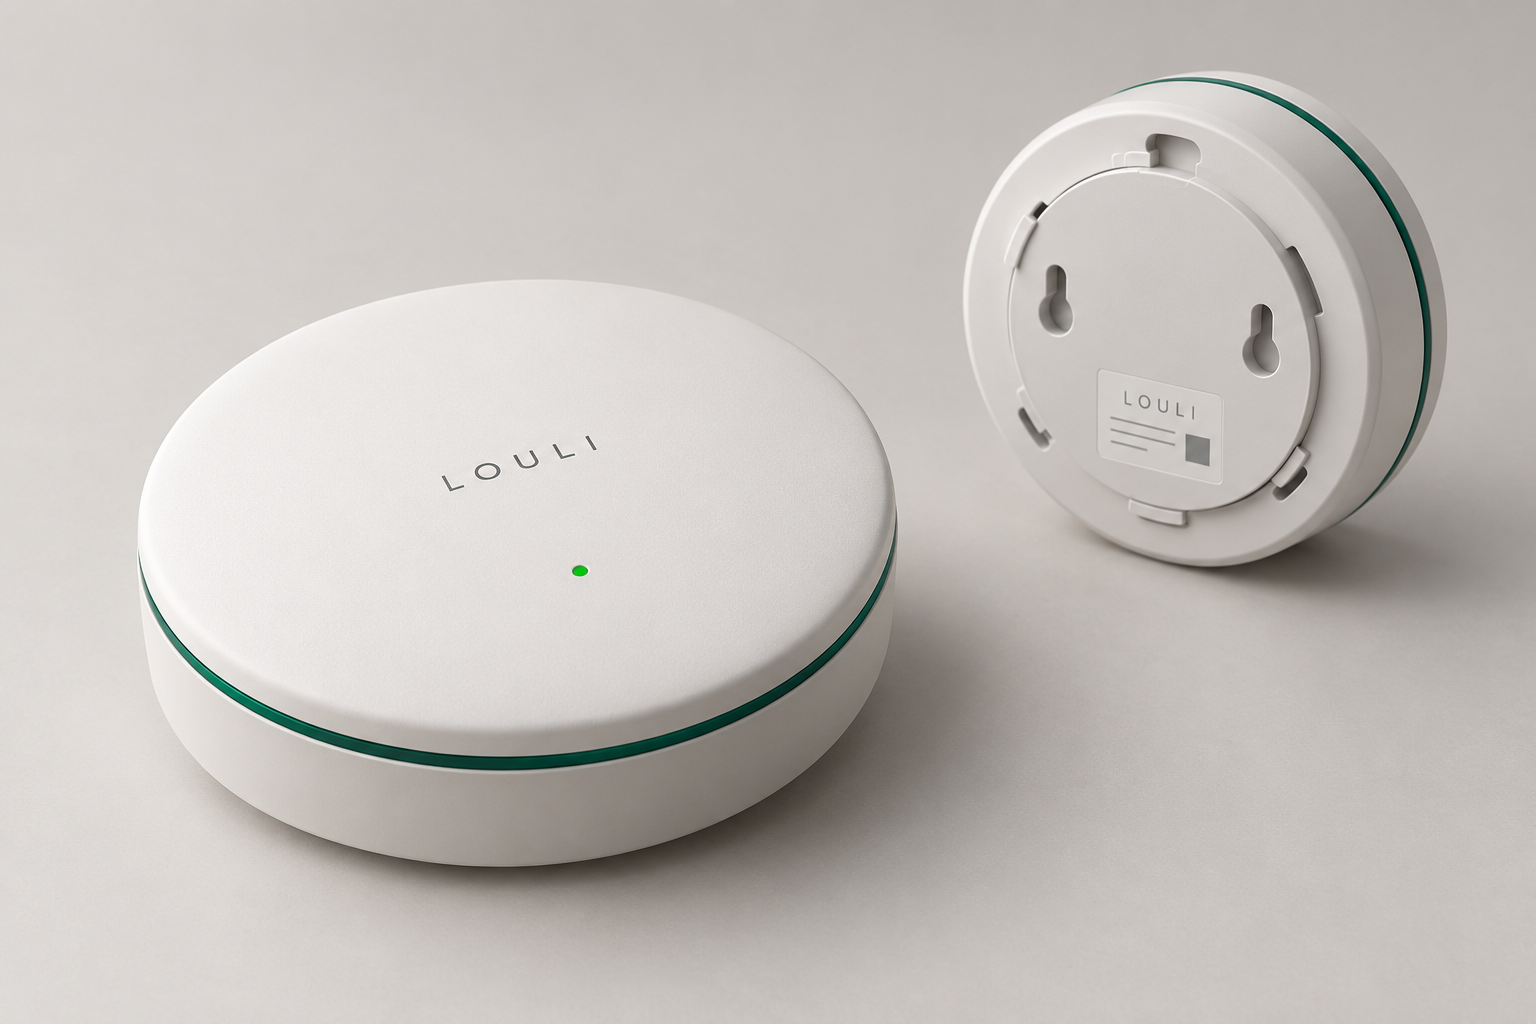
\includegraphics[width=\linewidth]{concept.png}
\note{本页为 AI 生成的产品概念图，非实物照片。目标外形为直径 70 mm、厚度 20 mm；尺寸、材料、灯光与安装结构均待机械和功耗验证。}
\vspace{3mm}
\par
\begin{tabularx}{\linewidth}{@{}p{30mm}X@{}}\toprule
外观方向 & 哑光白色圆盘、绿色接缝装饰、低存在感状态灯。\\
部署场景 & 楼层入口、走廊转角、服务台与目的地附近的固定点位。\\
当前阶段 & 网页侧 BLE + WiFi + PDR + EKF 为仿真展示；本稿不代表硬件已经完成。\\
产品承诺边界 & 不宣称已取得整机认证、达到定位精度或实现电池寿命。\\\bottomrule\end{tabularx}\par
\newpage
\kicker{02 / SYSTEM BOUNDARY}\titleline{信标广播身份，手机计算位置。}
固定信标周期广播标识与配置数据。手机结合信号观测、惯性传感器、楼层地图与算法估计位置；网页当前可展示这些过程的仿真。

\vspace{3mm}
\begin{tikzpicture}[every node/.style={font=\small},box/.style={draw=green,rounded corners,fill=green!6,text width=42mm,minimum height=19mm,align=center}]
\node[box] (b) at (0,0) {固定 BLE 信标\\ID / 广播参数};
\node[box] (p) at (5.6,0) {手机接收与计算\\RSSI / PDR / 融合};
\node[box] (m) at (11.2,0) {地图与服务\\导航 / 配置记录};
\draw[->,thick,green] (b)--(p);\draw[<->,thick,green] (p)--(m);
\end{tikzpicture}

\vspace{4mm}
\par
\begin{tabularx}{\linewidth}{@{}p{35mm}X@{}}\toprule
信标应承担 & 固定广播标识；发射功率与广播周期配置；维护模式；电池电压采样候选；固件版本管理。\\
手机侧承担 & BLE扫描、权限与后台行为适配；信号滤波；手机IMU步态与方向推算；定位融合与导航提示。\\
平台侧承担 & 信标ID与地图坐标绑定；配置台账；现场标定；维护记录与数据审计。\\
本版不内置 & WiFi、GPS、摄像头、IMU、蜂窝联网或持续在线网关。WiFi观测来自手机或既有设施。\\\bottomrule\end{tabularx}\par
\vspace{4mm}
\textbf{候选参数与验证要求}
\begin{itemize}
\item 广播协议先选 iBeacon 兼容格式或自定义广播；现场需核对手机平台与第三方配置工具的支持。
\item 可从 500--1000 ms 广播周期、0 dBm 发射功率开始试验；这些是测试起点，不是最终性能规格。
\item LED 仅在配置、检查时短闪；正常广播时关闭。数据帧可考虑电池电压，但电压与剩余电量的映射需实测。
\item 持续 BLE 扫描和手机 IMU 数据需要移动端原生能力或适用 SDK；普通网页仿真不能直接证明真实手机扫描链路。
\end{itemize}
\note{BLE RSSI 受遮挡、人体、楼层串扰与手机差异影响。定位效果需要现场走测；厂商广播距离不能换算为导航精度，也不能直接确定点位间距。}
\newpage
\kicker{03 / MECHANICAL CONCEPT}\titleline{可维护的六层结构。}
\begin{minipage}[t]{0.35\linewidth}\vspace{0pt}
\textbf{由上至下的概念结构}
\begin{enumerate}[leftmargin=1.4em,itemsep=8pt]
\item 白色上盖与导光柱
\item 绿色装饰接缝环
\item 圆形载板与 BLE 模组
\item CR2477 与电池座
\item 下壳与维护开口
\item 可拆安装底板
\end{enumerate}
\textbf{机械约束}

目标壳体 $\varnothing70\times20$ mm，圆形 PCB 约 $\varnothing50$ mm。CR2477 本体高约 7.7 mm，模组高约 2.2 mm；叠加电池座、PCB、外壳壁厚与间隙后，20 mm 需进一步校核。

电池置于 PCB 下方；模组天线位于板边，电池与金属件避开天线区。留空尺寸按最终模组数据手册。
\end{minipage}\hfill
\begin{minipage}[t]{0.62\linewidth}\vspace{0pt}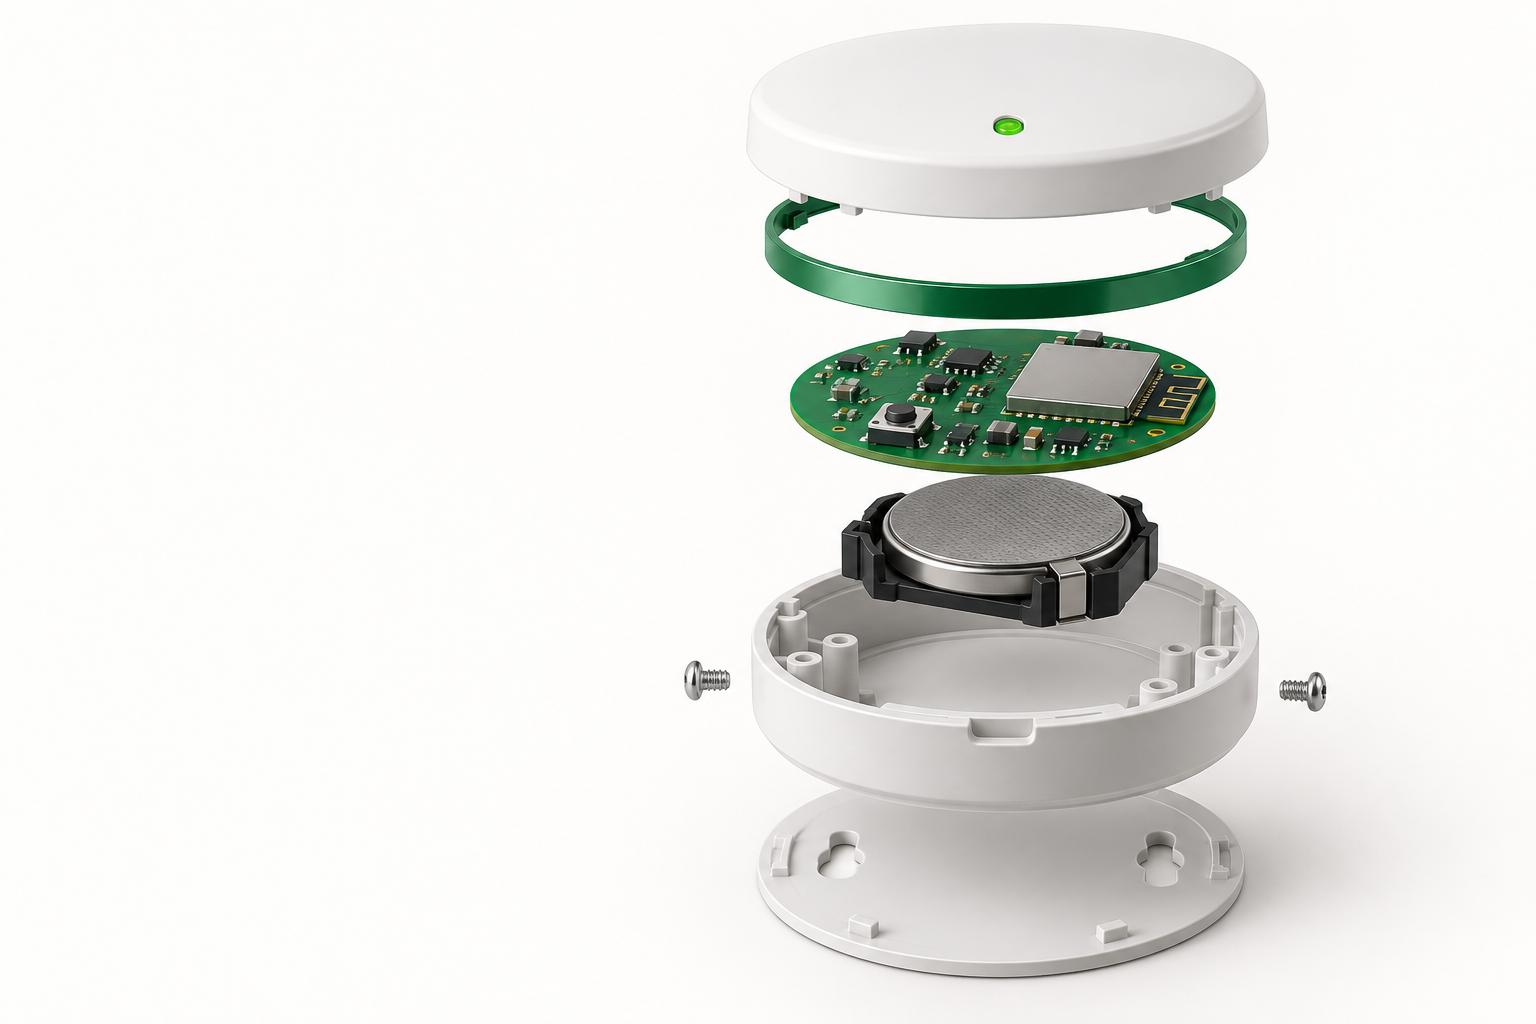
\includegraphics[width=\linewidth,height=160mm,keepaspectratio]{exploded.png}\end{minipage}
\note{AI 爆炸图仅说明装配关系，不对应实际 PCB、模组天线形式或公差。绿色环为外观件，非密封承诺；卡扣、电池连接与固定方式必须通过结构评审。未设定 IP 等级。}
\newpage
\kicker{04 / BOM AND BUDGET}\titleline{先选路线，再核算每台成本。}
\textbf{路线 A：现成信标样机，优先推进现场验证}

Minew E5 为候选，其厂商资料列出 BLE 广播、nRF52 系列与可更换电池。[1] 厂商产品单尺寸为 50$\times$20.5 mm，与楼里概念外观不同。[2] 采用原壳部署，不把现成设备塞进概念壳而改变天线环境。

工程预算：整机 80--150 元 / 台，安装标签 3--8 元 / 台；合计 \textbf{83--158 元 / 台}。此处为预留预算，非厂商报价，采购前需询价。

\textbf{路线 B：定制模组样机，后续推进品牌外观}
\small
\par
\begin{tabularx}{\linewidth}{@{}p{12mm}Xr r@{}}\toprule
编号 & 候选零件 / 服务（均为每台用量） & 数量 & 估算元\\\midrule
B01 & Raytac MDBT42Q-512KV2 BLE 模组 & 1 & 35--70\\
B02 & Panasonic CR2477 或等效一次电池 & 1 & 8--15\\
B03 & CR2477 低高度电池座 & 1 & 3--6\\
B04 & 约 50 mm 圆形双层 PCB & 1 & 8--15\\
B05 & 维护 / 配置按键 & 1 & 0.5--1.5\\
B06 & 绿色 LED 与导光组件 & 1套 & 1--3\\
B07 & 去耦、储能、保护与无源件 & 1套 & 3--6\\
B08 & 小批壳体与绿色装饰环 & 1套 & 12--25\\
B09 & 安装底板、辅料、资产标签 & 1套 & 3--8\\
B10 & 装配、烧录与单机检查 & 1台 & 8--18\\\midrule
 & \textbf{定制路线每台合计} & & \textbf{81.5--167.5}\\\bottomrule
\end{tabularx}\par\normalsize
\vspace{2mm}
\note{两条路线互相替代，不相加。CSV 提供零件、数量、理由、估算与来源。成本按小批工程预算建立，无供应商询价；具体料号与采购数量尚未锁定。}
\textbf{预算排除项}

以上不含运税、开发工具、原理图与 PCB 设计、固件研发、现场安装人工、模具、测试认证和备用设备。试点数量由走测决定；例如 12 台现成信标仅设备与辅料预算为 996--1896 元，不代表全场可部署方案或项目总价。
\newpage
\kicker{05 / PROTOTYPE TO PILOT}\titleline{把展示方案逐步变成可测的样机。}
\par
\begin{tabularx}{\linewidth}{@{}p{25mm}X X@{}}\toprule
阶段 & 工作与交付 & 进入下一步的条件\\\midrule
P0 现成设备 & 少量 E5；固定 ID；手机读取真实广播；建立点位台账与测试路线。 & 手机扫描链路可用；不同手机能识别 ID；地图坐标记录一致。\\
P1 小范围走测 & 测试遮挡、转角与楼层串扰；对比 BLE-only 与融合算法；记录偏差与成功到达率。 & 预先定义的场景验收标准通过；定位误差分布有记录。\\
P2 模组样机 & 模组开发板先验证广播与功耗，再做圆形 PCB、打印壳；完成电路与结构评审。 & 发射供电稳定；装配可维护；天线区符合资料；实测电流预算明确。\\
P3 OEM 试制 & 固定料号与固件；生产烧录、测试与追溯；按目标销售区域核对整机合规要求。 & 样机测试报告、工艺资料、供应商报价与售后流程完成。\\\bottomrule\end{tabularx}\par
\vspace{4mm}
\textbf{安装与维护建议}
\begin{itemize}
\item 优先墙面固定；点位高度、朝向和间距由现场测试选择。避开金属柜体与高干扰位置，不妨碍指示牌和消防设施。
\item 对医院环境，与设施管理方确认清洁剂、安装工艺与公共区域电池可接触性；壳体需有防误拆措施。
\item 每台标签记录：设备ID、楼栋/楼层/坐标、安装日期、固件版本、功率、广播周期、电池更换记录。
\item 更换电池后核对极性、标签与广播 ID；重新检查固定可靠性。CR2477 是一次电池，不设置充电口。
\item 巡检以实际电池监测与抽查确定周期；故障排查区分电量、设备丢失、信号遮挡、地图变更与手机权限问题。
\end{itemize}
\textbf{电池寿命如何估算}

使用测得的平均电流 $I_{avg}$ 与经过降额的可用容量 $C_{usable}$：$T\approx C_{usable}/I_{avg}$。需要计入广播周期、LED、配置连接、自放电、低温与电池截止电压。1000 mAh 是候选电池公称容量 [6]，不能作为整机寿命承诺。
\newpage
\kicker{06 / EVIDENCE AND OPEN ITEMS}\titleline{设计依据与待确认事项。}
\textbf{厂商主来源}\hfill{\small 访问日期：2026-10-07}
\small
\begin{enumerate}[leftmargin=1.5em,itemsep=8pt]
\item Minew E5 产品页：现成信标能力与可维护电池。\\\url{https://www.minew.com/product/e5-location-beacon/}
\item Minew E5 产品单：尺寸与广播格式。\\\url{https://www.minew.com/wp-content/uploads/2023/08/E5-poster.pdf}
\item Raytac MDBT42Q 系列规格（Version P）：模组尺寸与接口。\\\url{https://www.raytac.com/upload/download_files/38a8a4a0aff945d8484507d60058109b.pdf}
\item Nordic nRF52832 模组列表：MDBT42Q-512KV2 与芯片天线。\\\url{https://www.nordicsemi.com/Products/nRF52832/Modules}
\item Nordic nRF52832 产品页：BLE、GPIO、ADC 等 SoC 能力。\\\url{https://www.nordicsemi.com/products/nrf52832?lang=en}
\item Panasonic CR2477：3 V、公称 1000 mAh、24.5$\times$7.7 mm。\\\url{https://energy.panasonic.com/ap/business/products/lithium/coin-cr-standard/models/CR2477}
\end{enumerate}\normalsize
\vspace{2mm}
\textbf{评审前仍需完成}
\begin{itemize}
\item 原理图、PCB 布线、天线禁布区与供电瞬态验证。
\item 装配堆叠、公差、固定结构、电池防误拆与清洁兼容性。
\item 手机侧真实扫描、权限、后台策略与室内场景定位验收。
\item 最终料号、供货与成本询价；整机合规与量产测试方案。
\end{itemize}
\note{交付：6 页设计稿、可编辑 LaTeX、UTF-8 BOM CSV、概念图、爆炸图、来源清单与生成提示词。品牌视觉可用于方案展示，硬件能力以后续实测和最终工程资料为准。}
\end{document}
